% !TeX root = ../dokumentation.tex

\addchap{\langanhang}

{\Large
\begin{enumerate}[label=\Alph*.]
	\item Screenshot NameNode Web-Interface
	\item Programmablaufpläne
	\begin{enumerate}
		\item Main:main
		\item LFAConfiguration
		\item Bootstrap:init
		\item Driver:run
	\end{enumerate}
	\item List of CD Contents
	\item CD 
\end{enumerate}
}
\pagebreak

\section*{A. Screenshot NameNode Web-Interface}\label{sec:ScreenNameNodeWeb}
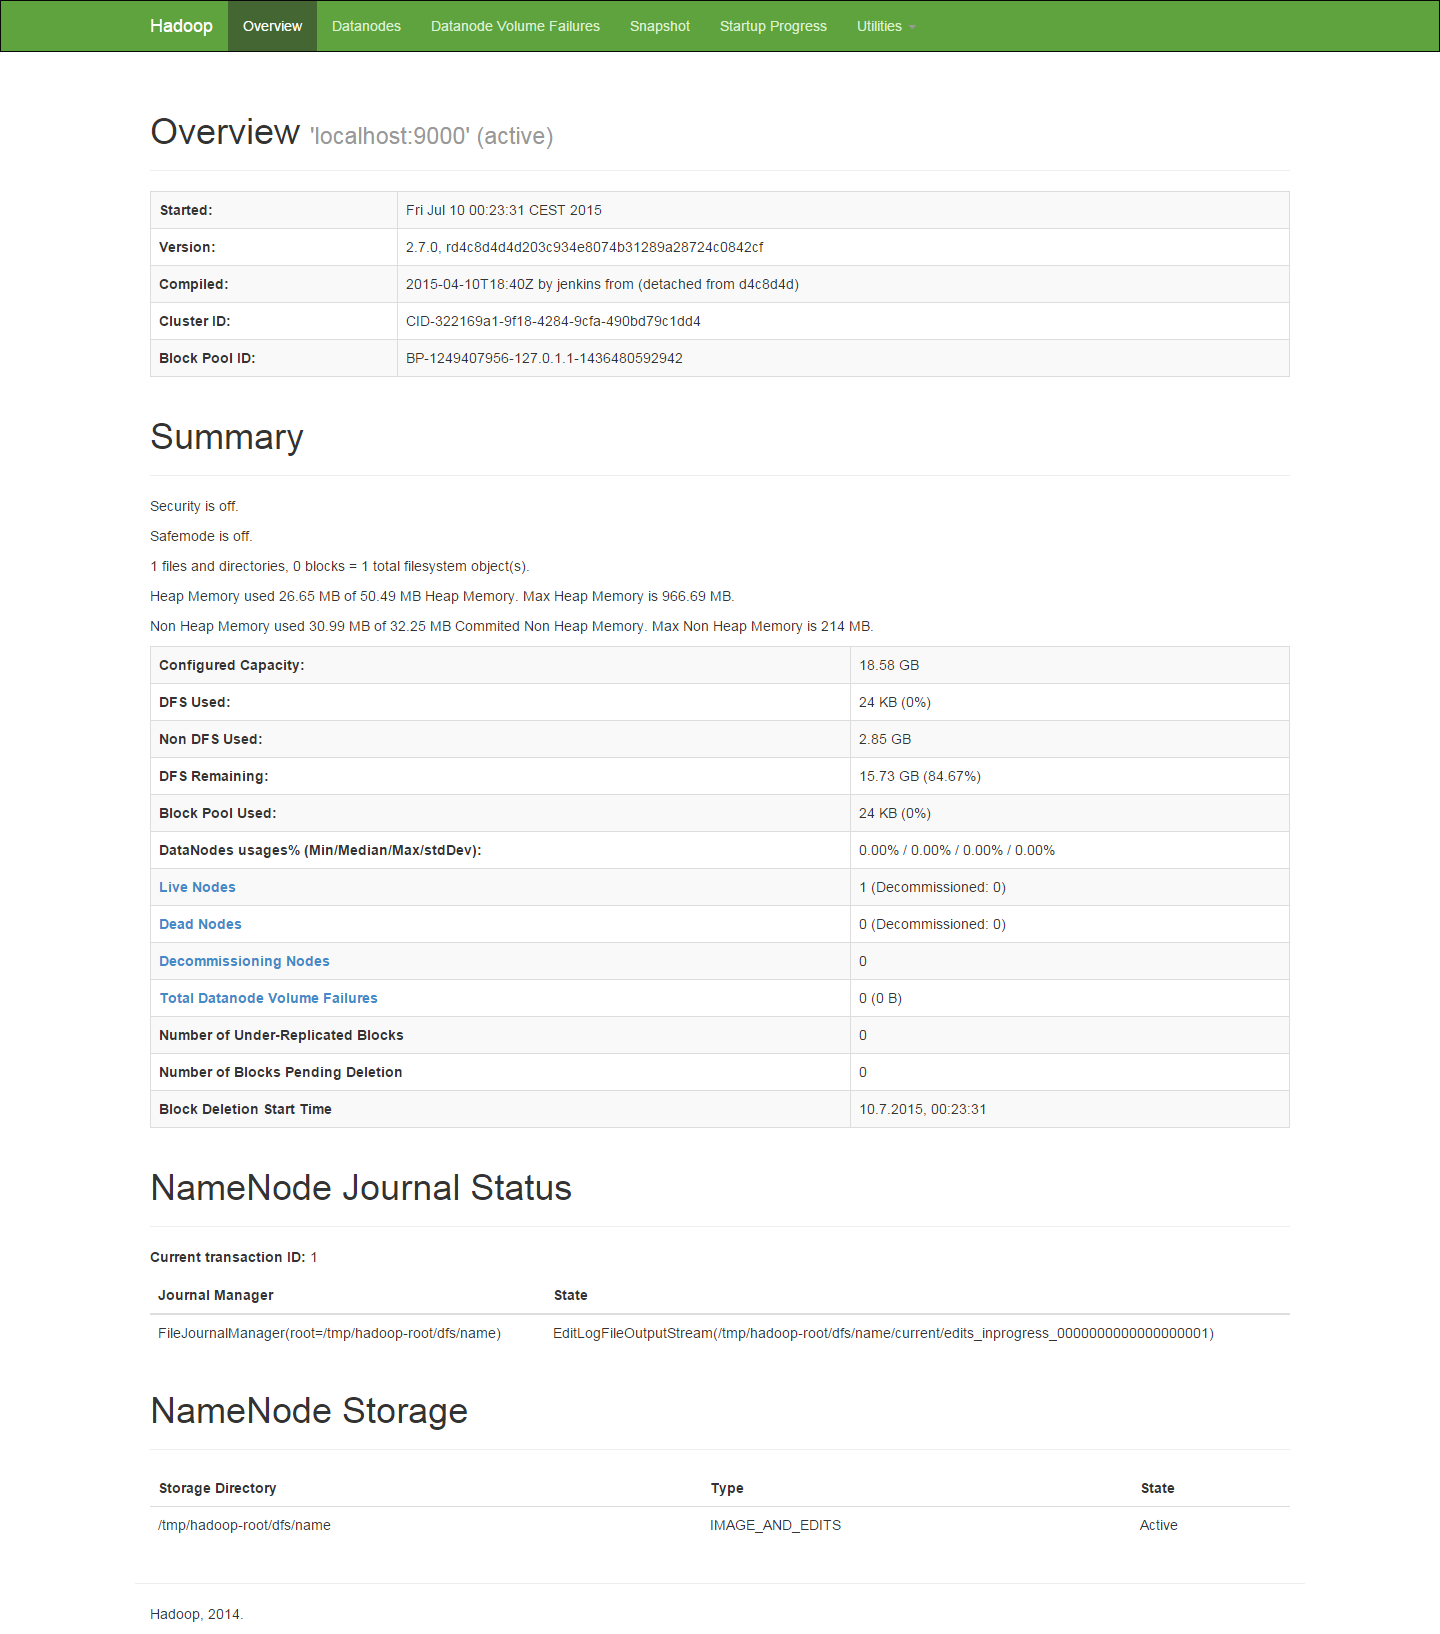
\includegraphics[width=1\textwidth]{NameNodeWebInterface.png}
\pagebreak

\section*{B. Programmablaufpläne}

\subsection*{B.a Main:main}\label{subsec:PAPMainMain}
\centering
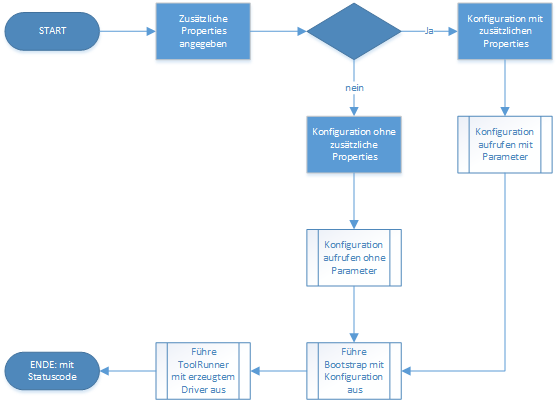
\includegraphics[scale=1]{PAP_Main_main.png}
\pagebreak

\subsection*{B.b LFAConfiguration}\label{subsec:PAPLFAConfiguration}
\centering
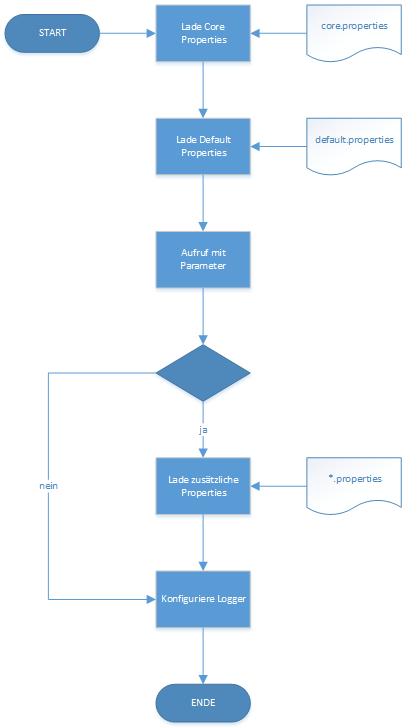
\includegraphics[scale=1]{PAP_LFAConfiguration.png}
\pagebreak

\subsection*{B.c Bootstrap:init}\label{subsec:PAPBootstrapInit}
\centering
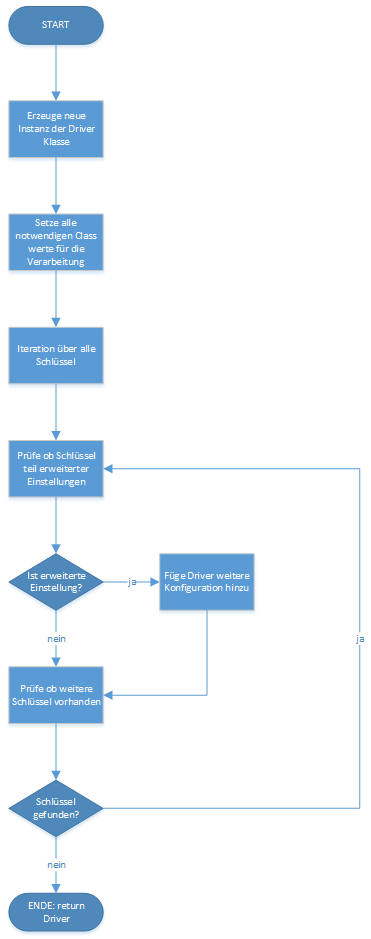
\includegraphics[scale=.9]{PAP_Bootstrap_init.png}
\pagebreak

\subsection*{B.d Driver:run}\label{subsec:PAPDriverRun}
\centering
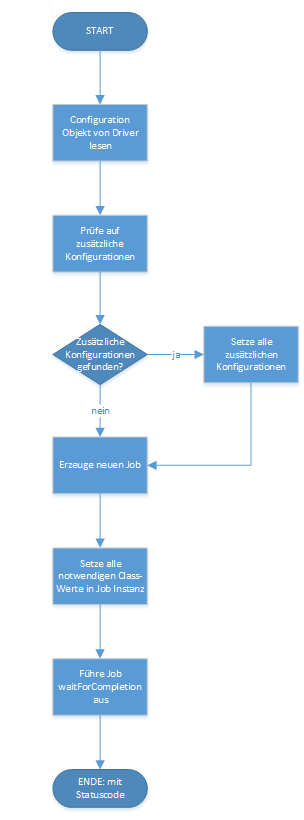
\includegraphics[scale=1]{PAP_Driver_run.png}
\pagebreak

\section*{B. List of CD Contents}
\begin{tabbing}
	mm \= mm \= mmmmmmmmmmmmmmmm \= \kill
	$\vdash$ \textbf{Sourcecode/} \\ 
	| \> $\vdash$ \textbf{conf/} \> \> \\
	| \> $\vdash$ \textbf{src/} \\
	| \> $\vdash$ \textbf{target/} \\
	| \\
	$\vdash$ \textbf{Präsentation/} \\
	| \>  -- praesentation.pptx \\
	| \>  -- praesentation.pdf \\
	| \\
	$\vdash$ \textbf{Testfiles/} \\ %\llcorner
	| \>  -- Aufgabenstellung.pdf\\
	| \>  -- Studienarbeit2.pdf\\
	| \\
	$\vdash$ \textbf{Latex-Files/} \> \> \> $\Rightarrow$ \textit{editable \LaTeX~files and other included files for this report}\\ %\llcorner
	\>  $\vdash$  \textbf{ads/}   	\> \> $\Rightarrow$ \textit{Front- and Backmatter}\\
	\>  $\vdash$  \textbf{content/}  \> \> $\Rightarrow$ \textit{Main part}\\
	\>  $\vdash$  \textbf{images/}   \> \> $\Rightarrow$ \textit{All used images}\\
	\>  $\vdash$  \textbf{lang/}  \> \> $\Rightarrow$ \textit{Language files for \LaTeX~template}\\ %\llcorner
\end{tabbing}
